\documentclass[twocolumn]{aastex631}
\received{\today}
\shorttitle{Giant Planet Formation}
\graphicspath{{figures/}}

\usepackage{lipsum}
\usepackage{physics}
\usepackage{multirow}
\usepackage{xspace}
\usepackage{natbib}
\usepackage{fontawesome5}
\usepackage{xcolor}
\usepackage{wrapfig}
\usepackage[figuresright]{rotating}

% remove indents in footnotes
\usepackage[hang,flushmargin]{footmisc} 

\newcommand{\todo}[1]{{\color{red}{[TODO: #1}]}}
\newcommand{\needcite}{{\color{magenta}{(needs citation)}}}
\newcommand{\placeholder}[1]{{\color{gray} \lipsum[#1]}}

% custom function for adding units
\makeatletter
\newcommand{\unit}[1]{%
    \,\mathrm{#1}\checknextarg}
\newcommand{\checknextarg}{\@ifnextchar\bgroup{\gobblenextarg}{}}
\newcommand{\gobblenextarg}[1]{\,\mathrm{#1}\@ifnextchar\bgroup{\gobblenextarg}{}}
\makeatother

\begin{document}

\title{{\huge Giant Planet Formation}\\\vspace{0.15cm}ASTR558 Final Project}

% affiliations
\newcommand{\UW}{Department of Astronomy, University of Washington, Seattle, WA, 98195}

\author[0000-0001-6147-5761]{Tom Wagg}
\affiliation{\UW}

\correspondingauthor{Tom Wagg}
\email{tomwagg@uw.edu}

\begin{abstract}
    There are currently two main theories for the formation of giant planets, core accretion and gravitational collapse. Core accretion can explain the formation of most planets but for more massive planets that are formed far from their host star, gravitational collapse is needed to explain their existence. In this paper we explain the processes involved in each theory as well as their relative merits and limitations. We additionally discuss recent work on different methods for constraining giant planet formation and highlight some major unsolved questions.
\end{abstract}

\keywords{}

\section{Key Concepts}

In this section, we explain the key concepts behind the two main theories of giant planet formation. At the end of the section, Figure~\ref{fig:formation_diagram} provides a schematic illustration and summary of the two formation channels that we discuss.

\subsection{Core Accretion}

At its simplest level, core accretion is where a central rocky core is formed and then accretes gas until it reaches a critical core mass and forms a giant planet \citep{Pollack+1996}.

The formation occurs in three phases, which can be seen in Figure~\ref{fig:planet_growth}. In the first phase, the planet is formed primarily of solid material and continuously accretes planetessimals at a higher rate than gas until the planet clears its ``feeding zone'', marking the end of the first phase. At this point the core of the planet has formed and now the planet slowly accretes gas in an envelope. This gas is accreted from a sphere of radius \citep{Bodenheimer+2013}
\begin{equation}
    R = \min \{ R_{\rm Bondi}, R_{\rm Hill} \}
\end{equation}
where $R_{\rm Bondi}$ is the Bondi radius, defining the maximum distance inside which gas can be bound to the core and $R_{\rm Hill}$ is the Hill radius, defining the radius in which the main gravitational influence is the planet. See Appendix~\ref{app:maths} for a derivation of expression for each of these radii.

The third phase of core accretion begins as the planetary core exceeds the critical core mass, resulting in rapid envelope contraction that leads to fast accretion of gas and thus planet mass growth. This finally results in a giant planet.

\subsubsection{Critical core mass}

During Phase 2 of formation via core accretion, slow accretion of gas and solids onto the core increases the envelope mass over time. For a given core mass, there exists an envelope mass above which hydrostatic equilibrium cannot be satisfied, which triggers the collapse of the envelope onto the core and therefore beginning of Phase 3.

This critical core mass can be derived using some basic assumptions about the locations of convective and radiative zones \citep{Stevenson+1982,Lissauer+2009}. Previous work assumed that the envelope was fully radiative but a more accurate assumption is that there is an innermost convective zone and outermost radiative zone. The combination of these zones gives that the critical core mass is simply
\begin{equation}
    M_{c} = \frac{1}{2} M
\end{equation}
implying that once the core mass accounts for half of the overall planet mass, rapid contraction will occur and Phase 3 of formation begins.

\begin{figure}
    \centering
    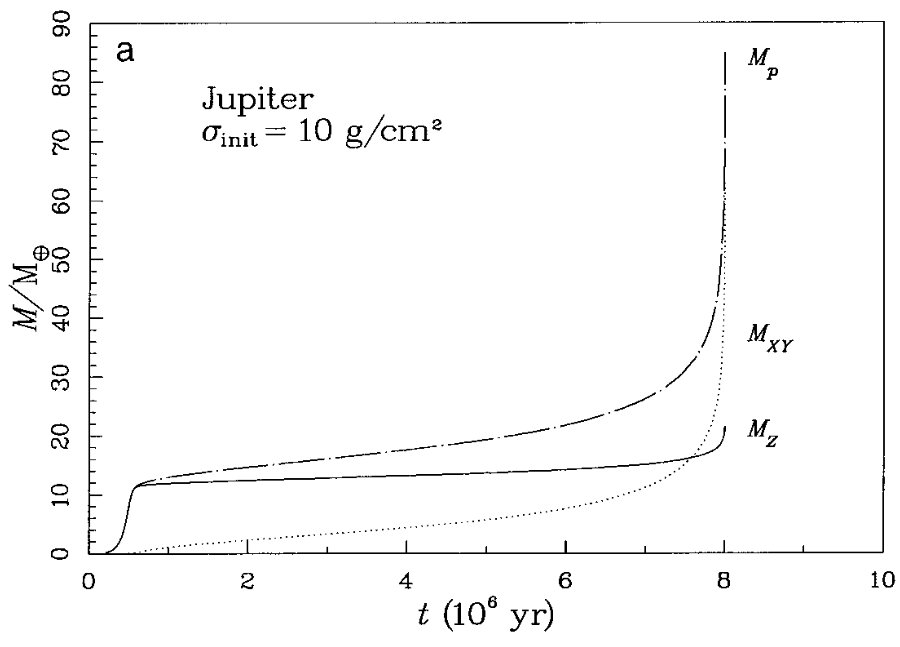
\includegraphics[width=\columnwidth]{pollack_fig_1.png}
    \caption{Figure 1 of \citet{Pollack+1996}. Planet mass as a function of time in which the three phases of core accretion are evident. Phase 1 is rapid early accretion of solids ($\sim$$0$--$0.4 \unit{Myr}$), Phase 2 is slow accretion onto the core ($\sim$$0.4$--$7.5 \unit{Myr}$) and Phase 3 is rapid final accretion once the critical core mass is exceeded ($\sim$$7.5$--$8 \unit{Myr}$). The different curves show the masses of different compositions.}
    \label{fig:planet_growth}
\end{figure}

\subsubsection{The end of accretion}

A giant planet formed via core accretion will finish its formation once there is no gas left for accretion. This termination occurs once the gas in the surrounding protoplanetary disc is dispersed (mainly by photo-evaporation). Prior to this dispersal, the accretion of a planet can also stall once it forms a gap in the protoplanetary disc after the end of Phase 3. This means that you can form different sorts of planets depending on what phase of formation they were in once the the gas in the disc is dispersed.

\citet{Lissauer+2009} showed that Saturn's mass is around the maximum for disc-limited accretion, whereas Neptune and Uranus were slower to form and would still have been on Phase 2 when the gas in the disc dispersed. The final planet mass therefore clearly depends on the star (specifically how luminous it is and how quickly it evolves) in addition to the planet location, disc density and other initial planet properties.

\subsubsection{Timescale limits}

The timescale on which core accretion occurs is strongly dependent on the distance of the planet from its host star. This means that, if we assume that all planets are formed via core accretion, one would expect that at larger distances the planets' masses would decrease (since they have less time to accrete and may not even reach Phase 3).

However, this is not what is seen observationally. In Figure~\ref{fig:demographics} we show a distribution of detected planets, plotting their separation against mass. It is evident that there is an abundance of large mass-large separation planets that couldn't possibly have been formed via core accretion. This leads to the second theory of giant planet formation - gravitational collapse.

\begin{figure}[tb]
    \centering
    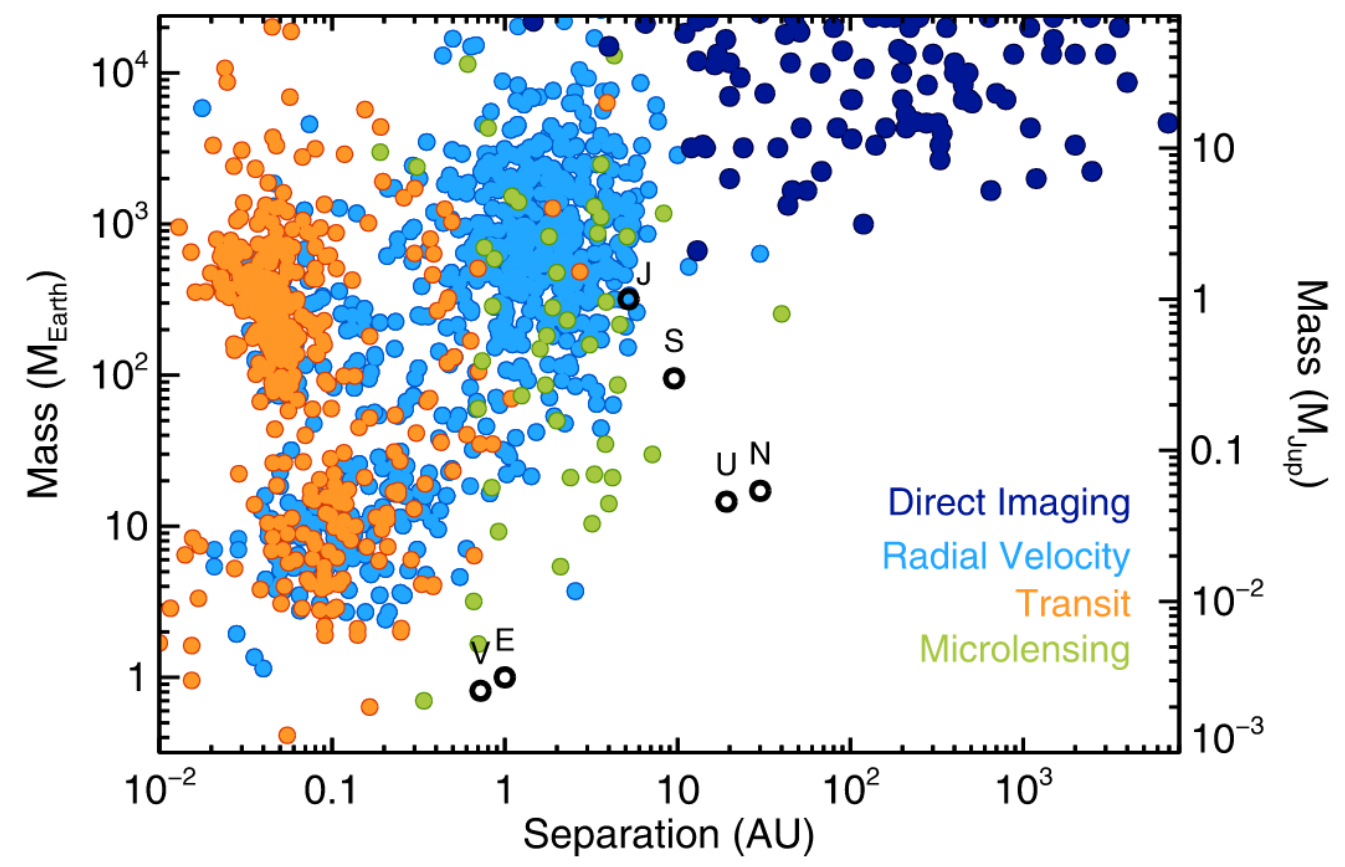
\includegraphics[width=\columnwidth]{exoplanet_demographics.png}
    \caption{Figure 13 from \citet{Bowler+2016}. Demographics of detected exoplanets, highlighting the large number of directly imaged planets that are far from their star whilst being very massive. These planets could not have been formed via core accretion.}
    \label{fig:demographics}
\end{figure}

\subsection{Gravitational collapse}

Often also referred to as disc instability or direct collapse, gravitational collapse is a formation mechanism that has been theorised for many years \citep{Kuiper+1951,Cameron+1982}, even before core accretion was more generally accepted. The idea is similar to the formation of a star, a gravitational instability occurs in the protoplanetary disc due to some perturbation, which leads to the formation of a self-gravitating collection of gas that eventually becomes the giant planet.

Core accretion has been more popular for a long time but more recently gravitational collapse has been necessary to explain more massive planets far from their host stars and thus has been investigated in more detail \citep{Durisen+2007}.

The gravitational instabilities occur once the Toomre stability parameter \citep{Toomre+1964}
\begin{equation}
    \mathcal{T} = \frac{c_g \Omega}{\pi G \Sigma_g}
\end{equation}
exceeds some critical value which is usually 1, but can be up to 2 for non-axisymmetric perturbations \citep{Binney+1987}. These instabilities can persist for a couple of orbits and so can have enough time to contract and form gaseous planets \citep{Forgan+2017}. Figure~\ref{fig:fragmentation} shows the fragmentations that can occur in the disc and lead to gravitational collapse.

\begin{figure}
    \centering
    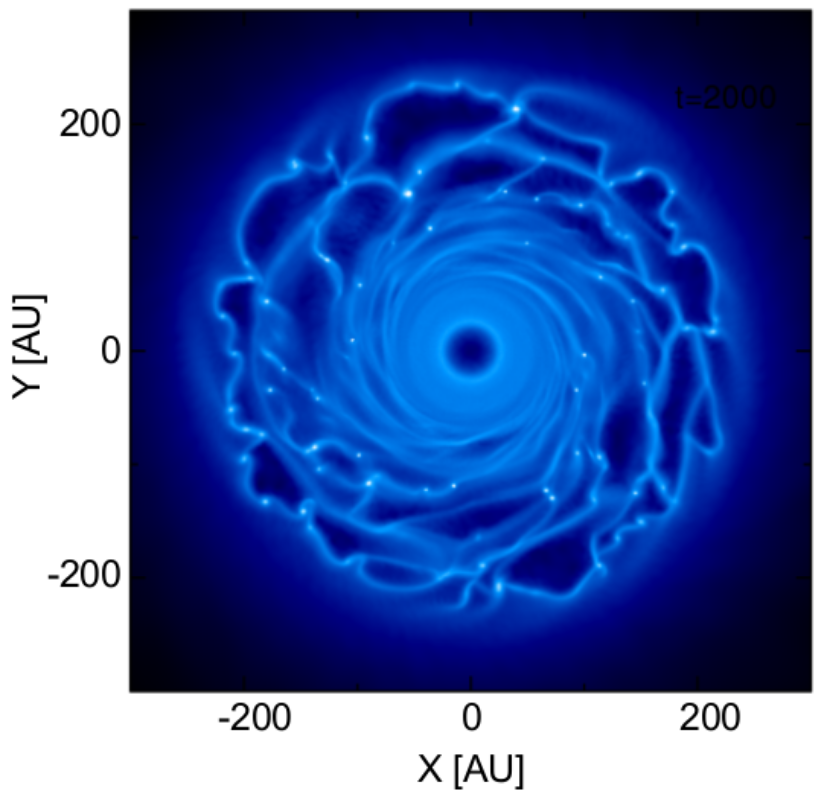
\includegraphics[width=\columnwidth]{fragmentation.png}
    \caption{Figure 4 from \citet{Forgan+2017}. A hydrodynamical simulation of a protoplanetary disc around a solar mass star. The colour indicates the column density and points of fragmentation can be seen as bright white spots.}
    \label{fig:fragmentation}
\end{figure}

The nature of this formation means that we'd expect planets formed in this to be enriched in heavy elements. This is because the perturbations that lead to gravitational instabilities sweep up dust and concentrate it prior to fragmentation \citep{Kratter+2016}. This can be a potential tracer for the formation history of a planet (more enriched giant planets are more likely to have been formed via gravitational collapse).

\subsubsection{Migration}

Another consideration is that the instabilities may not last long enough to form a planet reasonably close to the star. However, these planets can move closer to the star through planetary migration. Strong gravitational torques from the protoplanetary disc can change the planet's orbital angular momentum and thus cause it to migrate through the disc.

For a planet that has not opened a gap in the disc, it would experience \textit{Type I} migration for a large period of time \citep{Baruteau+2011}. The orbital decay scales with the mass of the planet and the density of the surrounding gas.

The main effect of the migration is of course that planets that form far from the star and reach much closer to the centre. However, the migration can also have strong effects on the planet itself, in particular its mass and size. At the start of migration a planet can be as large as its Hill radius but as it migrates the planet's outer layers can go beyond the Roche lobe of the planet and thus be stripped away. This unbinding of gas can strongly reduce the mass and size of planets as they migrate.

\begin{figure}[htb]
    \centering
    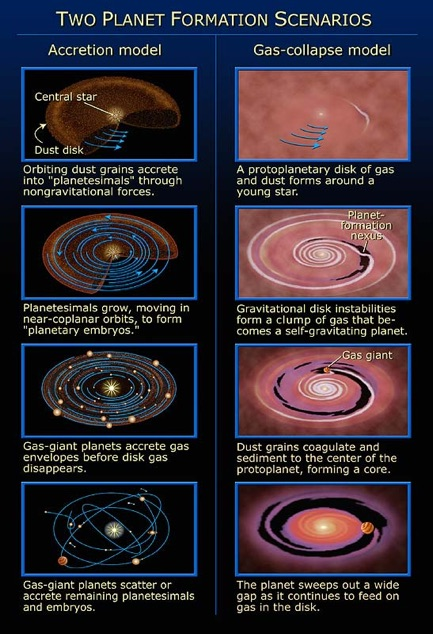
\includegraphics[width=\columnwidth]{channels_illustration.jpg}
    \caption{An illustration of different giant planet formation channels. (Credit: NASA and A. Feild (STScl))}
    \label{fig:formation_diagram}
\end{figure}

\section{Recent Research}

\subsection{Using the water content of sub-Neptunes to constrain giant planet formation}

\begin{figure*}
    \centering
    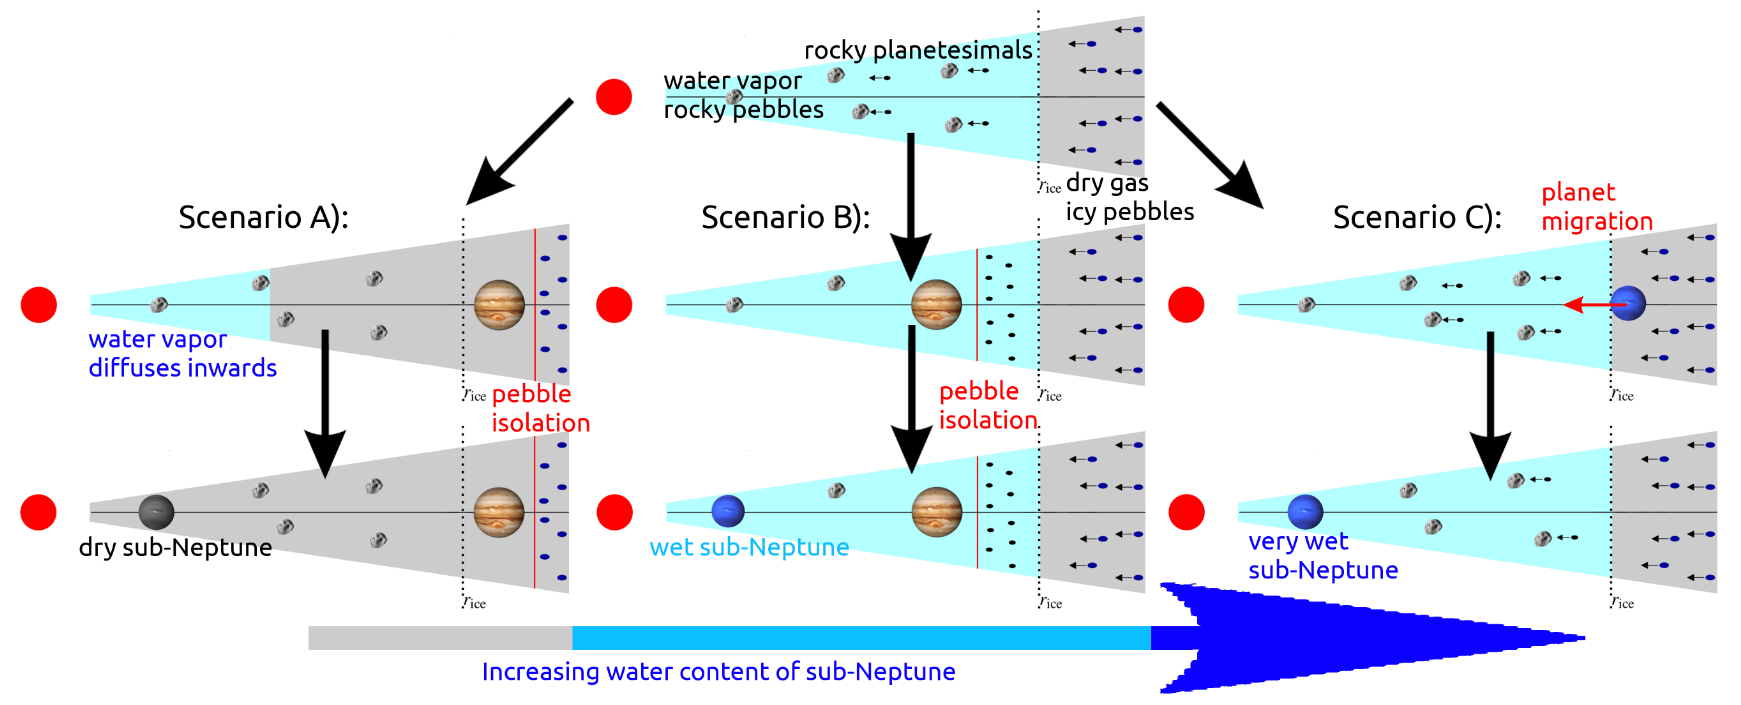
\includegraphics[width=\textwidth]{water_cartoon.png}
    \caption{Figure 1 from \citet{Bitsch+2021} showing 3 different potential formation scenarios in which the presence and location of a giant planet affects the water content of a sub-Neptune.}
    \label{fig:water}
\end{figure*}

\citet{Bitsch+2021} investigate how the water content of sub-Neptunes could be used to constrain giant planet formation. Inward moving water-rich pebbles from beyond the water-ice line can enrich the water content of sub-Neptunes as they evaporate and are accreted as water vapour by these planets. However, if a giant planet forms between the sub-Neptune and the water-rich pebbles it can block much of this accretion. Therefore the water content of these sub-Neptunes is directly related to presence (and therefore formation rate and timing) of giant planets.

Figure~\ref{fig:water} illustrates three different potential formation scenarios. In scenario A, a giant planet is formed beyond the water-ice line and its growing core exerts a pressure bump that prevents in the inward motion of water-rich pebbles. Additionally, the water vapour that was originally within the orbit of the giant planet quickly diffuses inwards and very little is accreted by the sub-Neptune thus resulting in a dry sub-Neptune.

In scenario B, the giant planet is instead formed within the water-ice line and so the water-rich pebbles, though still blocked from travelling beyond the giant planet, can evaporate and enrich the surrounding gas. This water vapour is then able to diffuse inwards past the giant planet (since gas accretion by giant planets is not 100\% efficient) and onto the sub-Neptune, resulting in a wet sub-Neptune.

Finally, in scenario C, no giant planet is formed and so the sub-Neptune accretes the water vapour from all inward drifting water-rich pebbles, resulting in a very wet sub-Neptune.

In the first scenario, the timing of the formation of the giant planet is critical. The core needs to be large enough early enough in the system formation to block the inward flux of water-rich pebbles in order to have a strong effect. This means that the formation time and original location of giant planets can be constrained by the water content of the sub-Neptunes.

\citet{Bitsch+2021} also discuss the effects of migration and the changing location of the water-ice line over time. The important takeaway is that it is the giant planet's position \textit{relative to the water-ice line} that determines the water content of the sub-Neptune.

\subsection{Evidence of an Upper Bound on the Masses of Planets formed via Core Accretion}

\citet{Schlaufman+2018} presents evidence for an upper bound on the masses of planets formed via core accretion. Their results rely on the assumption that core accretion is associated with metal-rich solar-type dwarf stars. They cross match exoplanets from the NASA exoplanet archive with stellar parameters from SWEET-Cat and collate a sample of 146 systems, arguing that selection effects are unlikely to be present in this sample.

\begin{figure}[htb]
    \centering
    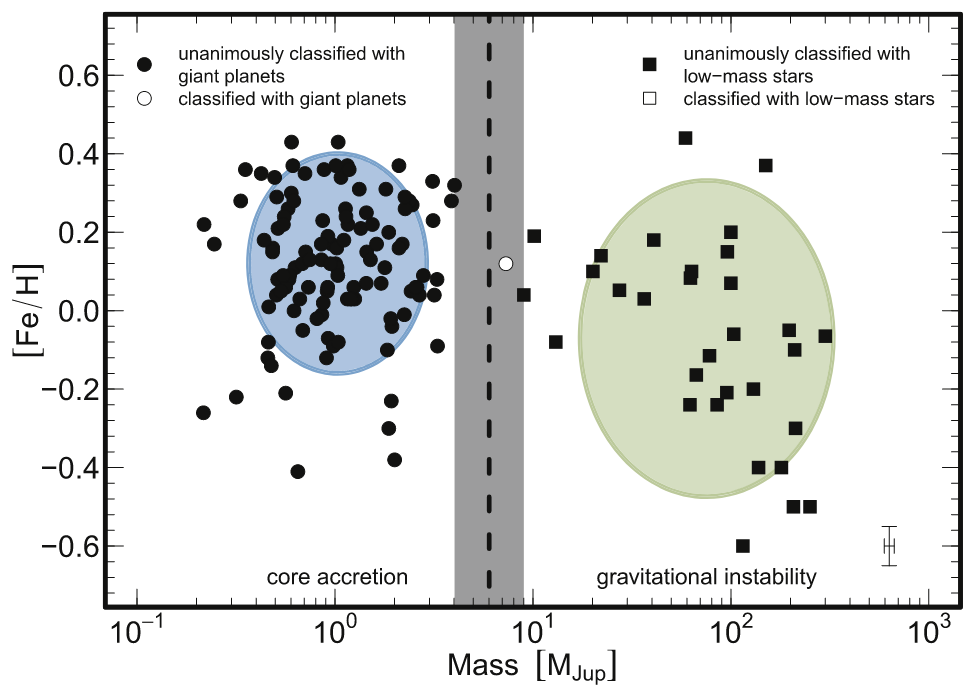
\includegraphics[width=\columnwidth]{max_core_acc_mass.png}
    \caption{Figure 1 of \citet{Schlaufman+2018}. This shows the masses and metallicities of the planets in the sample as well as their formation channel assigned by the aggregated clustering algorithms. The grey area and dashed line indicates the inferred maximum core accretion mass (found using a rolling window median).}
    \label{fig:max_mass}
\end{figure}

They use a series of clustering techniques to assign the planets to either core accretion or gravitational collapse in the metallicity--mass space. This is shown in Figure~\ref{fig:max_mass}. They infer that the grey area indicated on the plot is the maximum core accretion planet mass and therefore find it to be between 4 and 9 Jupiter masses.

I was also interested to read that the author felt that the definition of a planet should be based on its formation channel rather than its mass. They feel it is better to distinguish between planets and brown dwarfs with core accretion versus gravitational collapse rather than using the minimum mass needed to burn deuterium as the limit.

\subsection{Unsolved Questions}

Many core accretion models are currently unable to account for the importance and consequences of compositional gradients and internal mixing on the formation of giant planets \citep{D'Angelo+2018}.

There still exist many challenges with gravitational collapse as a theory for giant planet formation \citep{Forgan+2013}. In particular, it is still not clear what physical conditions are conducive for fragmentation of the disc and the survival of clumps after fragmentation (such that they can eventually form planets).

\section{Conclusion \& Summary}
We have described the two main formation mechanisms for giant planets: core accretion and gravitational collapse. The former can account for the formation of most planets but the latter is necessary for explaining the large planets that have been detected far from their host stars. There are limitations in both theories but they are still useful for explaining the formation of giant planets. We additionally discussed recent research on the potential use of the water content of sub-Neptunes for constraining giant planet formation as well as a paper providing evidence for an upper bound on the mass of planets formed via core accretion.

\bibliographystyle{aasjournal}
\bibliography{paper}{}

\appendix

\section{Derivation of Bondi and Hill Radii}\label{app:maths}

\subsection{Bondi Radius}
The Bondi radius is the maximum distance inside which gas can be bound to the core of the planet. The gas will be bound to the core if, in the frame of the core, its total energy becomes negative. This means that the gravitational potential energy needs to be greater than the total thermal energy and so we can write
\begin{equation}
    \frac{G M_c}{R} \ge \frac{1}{2} (v_{\rm rel}^2 + v_{\rm th}^2),
\end{equation}
where $M_c$ is the core mass, $R$ is the radius, $v_{\rm rel}$ is the relative velocity of the gas and the core and $v_{\rm th}$ is the thermal velocity of the gas. If we assume that the relative velocity is dominated by Keplerian shear \citep{D'Angelo+2018} then
\begin{equation}
    \abs{v_{\rm rel}} = R \Omega,
\end{equation}
where $\Omega = \sqrt{G M_* / a^3}$ is the angular orbital velocity. And the thermal velocity is given by
\begin{equation}
    v_{\rm th} = c_g \sqrt{8 / \pi}
\end{equation}
where $c_g$ is the speed of sound in the gas. The sound speed is often expressed as $c_g = H_g \Omega$, where $H_g$ is the pressure scale height of the disc. We can now plug this all into the original inequality (and make it an equality since we are solving for the Bondi radius) and, in the last line, assume that $R$ is much less than $H_g$.
\begin{align}
    \frac{G M_c}{R_{\rm B}} &= \frac{1}{2} (R^2 \Omega^2 + \frac{8}{\pi} H_g^2 \Omega^2) \\
    \frac{G M_c}{R_{\rm B}} &= \frac{G M_*}{2 a^3} (R^2 + \frac{8}{\pi} H_g^2) \\
    R_{\rm B} &= \frac{M_c}{M_*} \frac{2 a^3}{R^2 + \frac{8}{\pi} H_g^2} \\
    R_{\rm B} &\approx a \qty(\frac{M_c}{M_*}) \qty(\frac{a}{H_g})^2
\end{align}

\subsection{Hill Radius}
The Hill radius is a similar quantity but it is due to forces rather than energy. The radius is the maximum distance within which the main gravitational influence is the core of the planet. Let's assume a circular orbit in this case. Therefore, the Hill radius is found by equating the gravitational and centrifugal forces
\begin{equation}
    \frac{G M_p}{R_{\rm H}^2} - \frac{G M_*}{(a - R_{\rm H})^2} + \Omega (a - R_{\rm H}) = 0
\end{equation}
which we can equivalently write as follows using the definition of $\Omega$
\begin{equation}
    \frac{M_p}{R_{\rm H}^2} - \frac{M_*}{a^2} \qty(1 - \frac{R_{\rm H}}{a})^{-2} + \frac{M_*}{a^2} \qty(1 - \frac{R_{\rm H}}{a}) = 0
\end{equation}
Next we can take just the leading order to find
\begin{equation}
    \frac{M_p}{R_{\rm H}^2} - \frac{M_*}{a^2} \qty(1 + \frac{2 R_{\rm H}}{a}) + \frac{M_*}{a^2} \qty(1 - \frac{R_{\rm H}}{a}) = 0
\end{equation}
This gives the definition of the Hill radius as
\begin{equation}
    R_{\rm H} = a \qty(\frac{M_p}{3 M_*})^{1/3}
\end{equation}


\end{document}